\documentclass[xcolor=pdftex,x11names,table,hyperref]{beamer}

\usepackage{verbatim}
\usepackage{setspace}
\usepackage{url}
\usepackage{xcolor} % See documentation PDF at http://www.ctan.org/pkg/xcolor
\definecolor{darkgreen}{rgb}{0,0.3,0}
\definecolor{darkblue}{rgb}{.05,.05,.30}
\definecolor{lightgrey}{rgb}{0.65,0.65,0.65}
\usepackage{tikzsymbols}


\setbeamertemplate{section in toc}[sections numbered]
\setbeamertemplate{subsection in toc}[subsections numbered]
\setbeamertemplate{subsubsection in toc}[subsubsections numbered]
\usetheme{Singapore}
\setbeamertemplate{navigation symbols}{}
\setbeamertemplate{footline}{%
\vspace{0.0em}%
\hspace{0.5em}%
{\color[rgb]{.1,.1,.1} \insertframenumber{}~/~\inserttotalframenumber}
}

\newcommand{\code}[1]{{\color{darkgreen}\texttt{#1}}}
\newcommand{\detail}[1]{{\color{lightgrey}\small{}#1}}
\newcommand{\teeny}[1]{\scalebox{0.09}{#1}}
\newcommand{\tablecolors}{\rowcolors{2}{blue!12}{white}} % Cool table colors


\begin{document}

\title{Sequence to Sequence Models \\[1.5em]
 %
\includegraphics[width=0.5\textwidth]{images/kitten_string_flickr_albaraa.jpg} \\[-1.0em]
 %\small{Possibilities} \\[1.0em]
 %LT1 \\[1.0em]
 }
\author{\href{http://jon.dehdari.org}{Jon Dehdari}}
\frame{\titlepage}

\begin{frame}{Good Morning!}
	\begin{center}
	%\includegraphics[width=0.8\textwidth]{images/.jpg}
	\end{center}
\end{frame}


% Cho: It's all LMs! (ala doc brown)
% ?Joint model?

% Start with basic seq2seq model
% http://arxiv.org/abs/1409.3215 (Sutskever et al, 2014)
% can use final hidden layer to kinda represent entire sentence.  Shortcomings?
\begin{frame}{Sentence Vectors}
\begin{itemize}
	\item We've seen that words can be represented as vectors. Can sentences be represented as vectors? \pause
	\item Sure, why not? \pause How?  From the hidden state at the end of a sentence: \hspace{1.0em}
	$ \mathbf{h}_i = \phi_{\text{enc}} ( \mathbf{h}_{i-1}, \mathbf{s}_i ) $
		\small{ \detail{($\phi_{\text{enc}}$ = LSTM or GRU)} }
	\pause
	\begin{center} 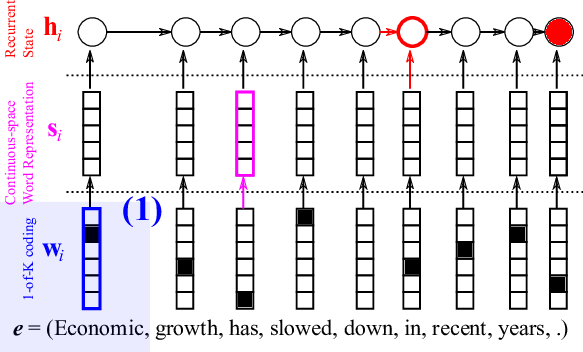
\includegraphics[width=0.63\textwidth]{images/cho_nvidia_fig-3_one-hot.png} \end{center}
	\pause
	\item Are they any good?  For Elman networks (SRNs), not so much.  For LSTMs or GRUs, yes, they're pretty good
\end{itemize}
\teeny{Image courtesy of \url{http://devblogs.nvidia.com/parallelforall/introduction-neural-machine-translation-gpus-part-2}}
\end{frame}

\begin{frame}{Sentence Vector Examples}
\hspace*{-3.0em}%
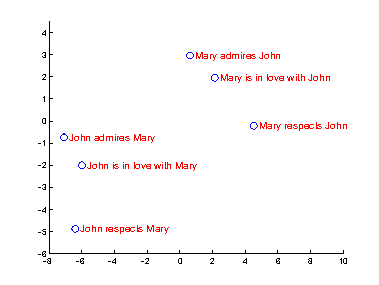
\includegraphics[width=0.60\textwidth]{images/sutskever-etal2014_fig2a.pdf}\hspace*{-1.0em}%
	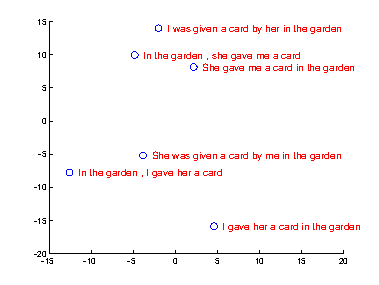
\includegraphics[width=0.60\textwidth]{images/sutskever-etal2014_fig2b.pdf}
\teeny{Images courtesy of \href{http://arxiv.org/abs/1409.3215}{Sutskever, et al (2014)}}
\end{frame}

% generate text from a vector (decoding)
\begin{frame}{Generating Sentences from Vectors}
\begin{itemize}
	\item We can also try to go the other direction, generating sentences from vectors
	\item How?  Use an RNN to \textbf{decode}, rather than \textbf{encode} a sentence: \hspace{1.0em}
		$ \mathbf{z}_i = \phi_{\text{dec}} ( \mathbf{z}_{i-1}, \mathbf{u}_{i-1}, \mathbf{h}_T ) $
\begin{center}
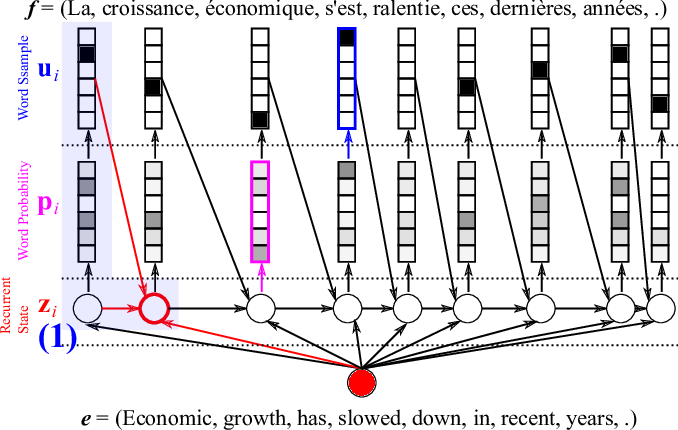
\includegraphics[width=0.60\textwidth]{images/cho_nvidia_figure7_internal-hidden-state.png}
\end{center}
	\item $\mathbf{h}_T$ ensures global sentence coherency (\& adequacy in MT); $\mathbf{u}_{i-1}$ ensures local fluency
\end{itemize}
\teeny{Image courtesy of \url{http://devblogs.nvidia.com/parallelforall/introduction-neural-machine-translation-gpus-part-2}}
\end{frame}



% http://devblogs.nvidia.com/parallelforall/introduction-neural-machine-translation-gpus-part-2/
% https://www.tensorflow.org/versions/master/tutorials/seq2seq/index.html
\begin{frame}{Using Neural Encoders \& Decoders to Translate}
\begin{itemize}
	\item We can combine the neural encoder and decoder of previous slides to form an \textbf{encoder-decoder model}
	\item This can be used for machine translation, and other tasks that map sequences to sequences
\begin{center}
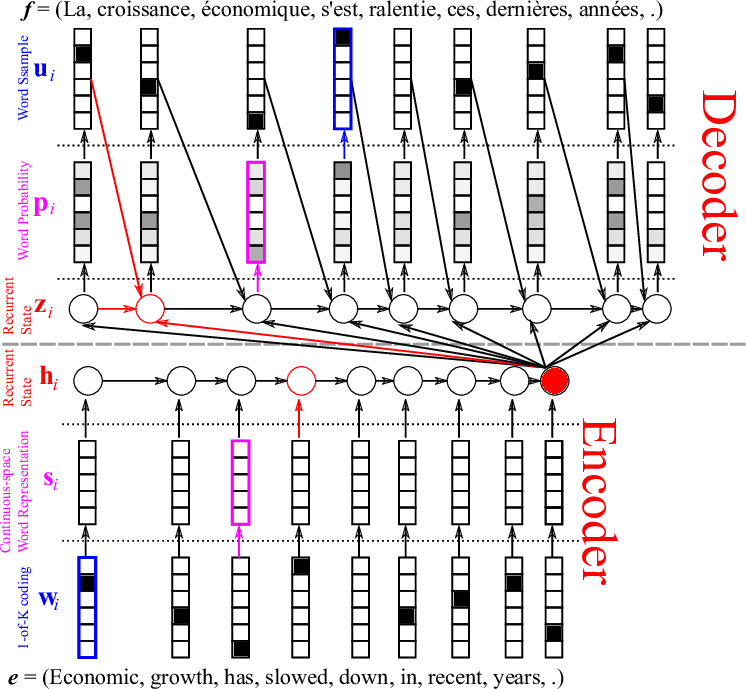
\includegraphics[width=0.40\textwidth]{images/cho_nvidia_fig-2_enc-dec.png}
\end{center}
	\pause
	\item Monolingual word projections (vectors/embeddings) are trained to maximize likelihood of next word
	\item Source-side word projections ($\textbf{s}_i$) in an encoder-decoder setting are trained to maximize target-side likelihood
\end{itemize}
\teeny{Image courtesy of \url{http://devblogs.nvidia.com/parallelforall/introduction-neural-machine-translation-gpus-part-2}}
\end{frame}


\begin{frame}{Bidirectional RNNs}
\begin{itemize}
	\item The basic encoder-decoder architecture doesn't handle long sentences very well
	\item Everything must fit into a fixed-size vector,
	\item and RNNs remember recent items better
	\pause
	\item We can combine left-to-right and right-to-left RNNs to overcome these issues
\begin{center}
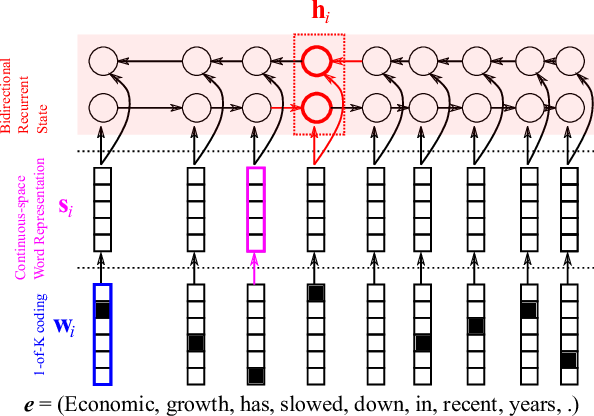
\includegraphics[width=0.60\textwidth]{images/cho_nvidia_fig-2_birnn.png}
\end{center}
\end{itemize}
\teeny{Image courtesy of \url{http://devblogs.nvidia.com/parallelforall/introduction-neural-machine-translation-gpus-part-3}}
\end{frame}


\begin{frame}{What if \ldots}
\begin{itemize}
	\item Even bidirectional encoder-decoders have a hard time with long sentences
	\item We need a way to keep track of what's already been translated and what to translate next
	\pause
\begin{center}

\includegraphics[width=0.40\textwidth]{images/keanu_what_if_nnet.jpg}
\end{center}
	\pause
	\item For neural nets, the solution is often more neural nets \ldots
\end{itemize}
\end{frame}


% see http://www.wildml.com/2016/01/attention-and-memory-in-deep-learning-and-nlp/
\begin{frame}{Achtung, Baby!}
\begin{itemize}
	\item Attention-based decoding adds another network ($\mathbf{a}$) that takes as input the encoder's hidden state ($\mathbf{h}$) and the decoder's hidden state ($\mathbf{z}$), and outputs a probability for each source word at each time step (when and where to pay attention) :\\
		$e_{i,j} = a(z_{i-1}, h_j) = v^{\top}_a \tanh (W_a s_{i-1} + U_a h_j) $

\begin{center}
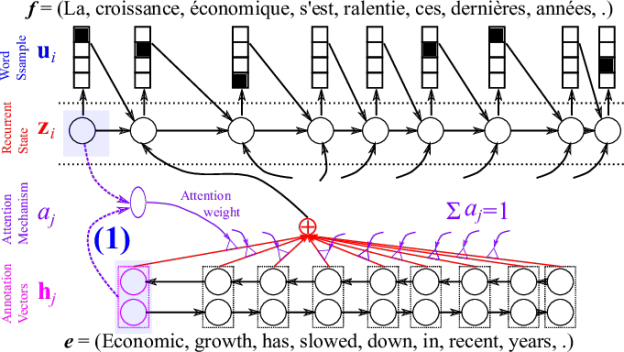
\includegraphics[height=0.43\textheight]{images/cho_nvidia_fig-3_attention.png}
\end{center}

	\pause
	\item The attention weights can also function as soft word alignments. They're trained on target-side MLE
\end{itemize}
\teeny{Image courtesy of \url{http://devblogs.nvidia.com/parallelforall/introduction-neural-machine-translation-gpus-part-3}}
\end{frame}



% see http://www.wildml.com/2015/09/recurrent-neural-networks-tutorial-part-1-introduction-to-rnns/
\begin{frame}{Image Caption Generation}
\begin{itemize}
	\item You can use attention-based decoding to give textual descriptions of images
\end{itemize}
\begin{center}
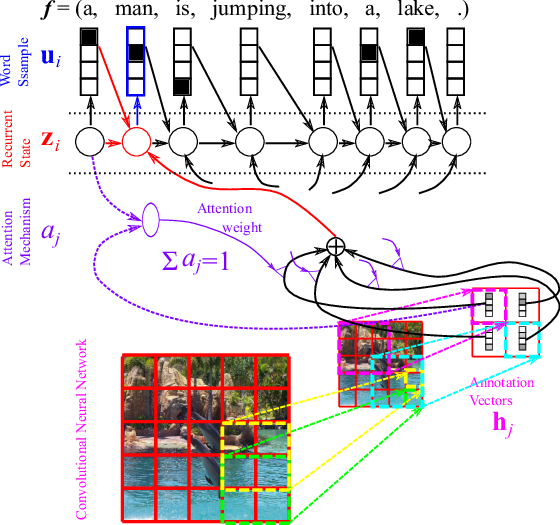
\includegraphics[height=0.71\textheight]{images/cho_nvidia_fig-8_image_caption.png}
\end{center}
\teeny{Image courtesy of \url{http://devblogs.nvidia.com/parallelforall/introduction-neural-machine-translation-gpus-part-3}}
\end{frame}

\begin{frame}{Image Caption Generation Examples}
\begin{center}
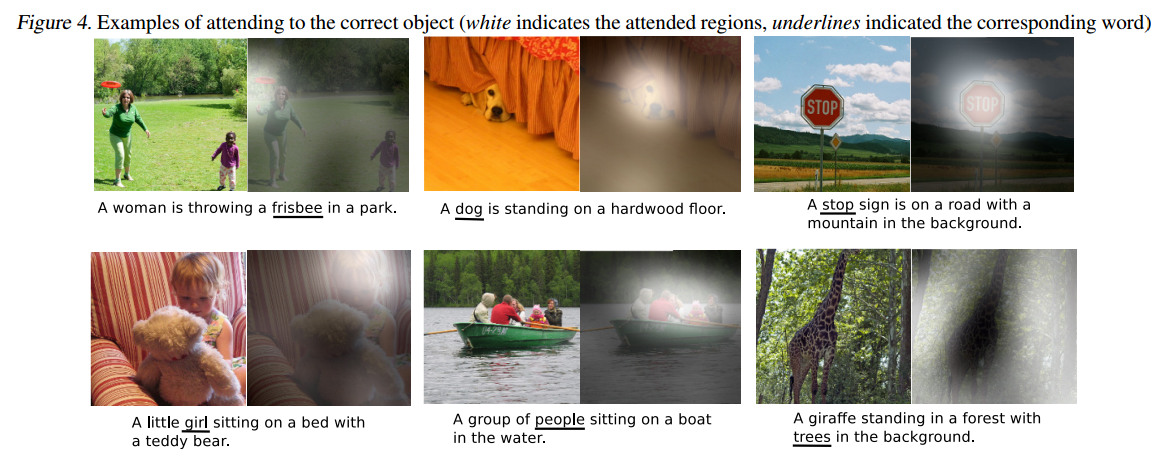
\includegraphics[width=1.07\textwidth]{images/xu-etal2015_icml_fig4.jpg}
\end{center}
\teeny{Images courtesy of \url{http://arxiv.org/abs/1502.03044}}
\end{frame}



\begin{frame}{Image Caption Generation, Step by Step}
\begin{center}
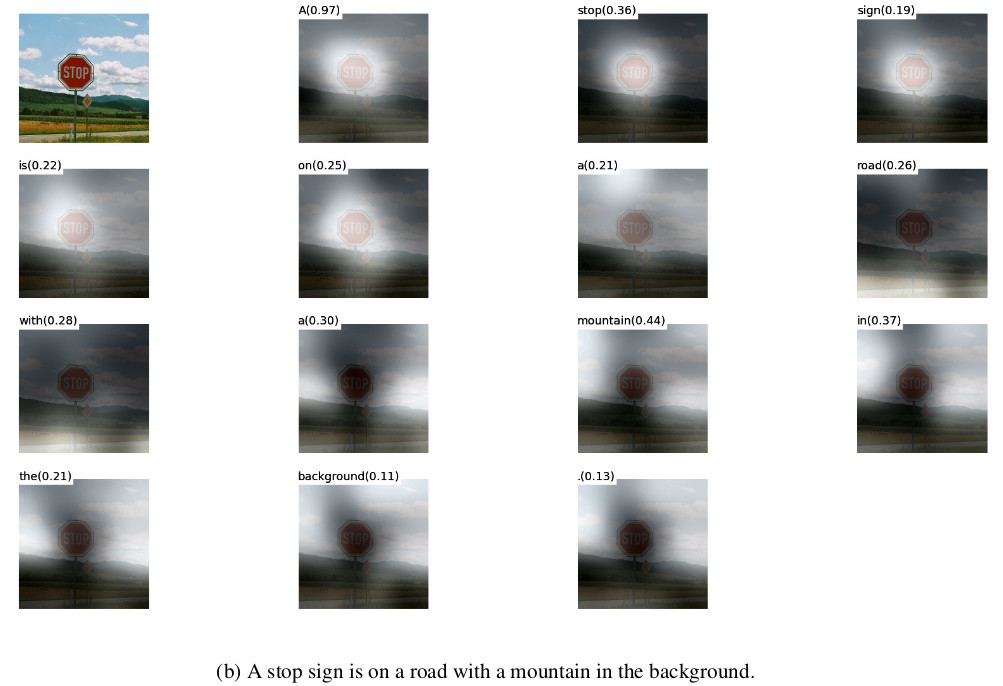
\includegraphics[width=0.90\textwidth]{images/xu-etal2015_icml_fig10b.jpg}
\end{center}
\teeny{Images courtesy of \url{http://arxiv.org/abs/1502.03044}}
\end{frame}






% \begin{frame}{}
% \begin{itemize}
% 	\item 
% 	\item 
% 	\item 
% \end{itemize}
% \end{frame}


\end{document}
